\documentclass{article}

% if you need to pass options to natbib, use, e.g.:
% \PassOptionsToPackage{numbers, compress}{natbib}

% ready for submission
\usepackage{aaai}

% to compile a preprint version, e.g., for submission to arXiv, add
% add the [preprint] option:
% \usepackage[preprint]{nips_2018}

% to compile a camera-ready version, add the [final] option, e.g.:
% \usepackage[final]{nips_2018}

% to avoid loading the natbib package, add option nonatbib:
% \usepackage[nonatbib]{nips_2018}

\usepackage[utf8]{inputenc} % allow utf-8 input
\usepackage[T1]{fontenc}    % use 8-bit T1 fonts
\usepackage{hyperref}       % hyperlinks
\usepackage{url}            % simple URL typesetting
\usepackage{booktabs}       % professional-quality tables
\usepackage{amsfonts}       % blackboard math symbols
\usepackage{nicefrac}       % compact symbols for 1/2, etc.
\usepackage{microtype}      % microtypography
\usepackage{amssymb}
\usepackage{natbib}
%% The amsthm package provides extended theorem environments
\usepackage{amsthm}
\usepackage{float}
\usepackage{sgame, tikz} % Game theory packages
\usepackage{caption} 
\usepackage{algorithm,algpseudocode}
\usepackage{makecell}
 \usepackage{multirow}
 \usepackage{graphicx}
\theoremstyle{definition}
\newtheorem{definition}{Definition}
\captionsetup{font=footnotesize}
\bibliographystyle{aaai}




% The \author macro works with any number of authors. There are two
% commands used to separate the names and addresses of multiple
% authors: \And and \AND.
%
% Using \And between authors leaves it to LaTeX to determine where to
% break the lines. Using \AND forces a line break at that point. So,
% if LaTeX puts 3 of 4 authors names on the first line, and the last
% on the second line, try using \AND instead of \And before the third
% author name.




\begin{document}

\title{Learning and Reputation under Monopoly and Duopoly: \\A Competing Bandits Approach}

\author{Guy Aridor\textsuperscript{1}, Kevin Liu\textsuperscript{2}, Aleksandrs Slivkins\textsuperscript{3},
Zhiwei Steven Wu\textsuperscript{4} \\
{\textsuperscript{1}Columbia University, Department of Economics}\\
{\textsuperscript{2}Columbia University, Department of Computer Science}\\
{\textsuperscript{3}Microsoft Research, New York, NY}\\
{\textsuperscript{4}University of Minnesota - Twin Cities, Department of Computer Science}
}
\maketitle

\begin{abstract}
We empirically study the interplay between \textit{exploration} and \textit{competition} - how systems that learn from interactions with users tradeoff between making potentially suboptimal choices in order to acquire new information and the reputational consequences of this exploration which potentially has adverse competitive effects. Our model considers competition for myopic users between two firms deploying multi-armed bandit algorithms that face the same underlying multi-armed bandit instance. The users select between the firms according to a reputation score, which is a function of the rewards past users have experienced from this firm.

We ask whether better algorithms are incentivized under varying degrees of competition. The environments we consider are a monopoly, a duopoly with one firm serving as an early entrant (a temporary monopoly), and a duopoly. We show that, under certain conditions, monopoly and duopoly do not incentivize the adoption of better learning algorithms due to the reputational costs of exploration, but that a temporary monopoly may incentivize the adoption of better learning algorithms. Additionally, we interpret our results as providing an alternative intuition behind the classic first-mover advantage which gives the incumbent firm both a data advantage and a reputational advantange. Finally, we ask whether in this setting the data advantage or the reputational advantage of the early entrant serves as stronger barriers to entry.
\end{abstract}

\section{Introduction}
\label{S:1}

Many modern online platforms simultaneously compete for users as well as learn from the users they manage to attract. For instance, Google Search and Bing compete for users in the search engine market yet at the same time need to experiment with their search algorithms to learn what algorithms work the best. This creates a tradeoff between \textit{exploration} and \textit{competition} since firms need to experiment with potentially sub-optimal options for the benefit of gaining information to make better decisions tomorrow while at the same time firms need to incentivize consumers to select them over their competitors today.

From a social welfare perspective it is better for firms to adopt ``better" learning algorithms and our main high-level question is asking under what levels of competition are firms incentivized to adopt ``better" learning algorithms. Our primary contribution is that in our model, even in the case of a duopoly, firms are not incentivized to adopt better learning algorithms but that allowing one firm to be a temporary monopolist will incentivize this firm to play a better learning algorithm. 

Unlike in the classic models in economics regarding the interplay between competition and innovation described in \citet{barro2004economic}, here we have no explicit R \& D cost. Rather, firms are not incentivized to experiment under duopoly because experimentation has an implicit relative \textit{reputational} cost compared to the myopic alternative and, in our model, consumers only care about the reputation of a firm. Thus, competition disincentivizes experimentation by firms precisely because competition forces firms to take actions in order to incentivize consumers to select them over their competitors and, as a result, by allowing a firm to be a temporary monopolist the firm can experiment without worrying about the reputational consequences. Our findings give an alternative intuition to the empirically documented inverse-U relationship between competition and innovation discussed in \citet{aghion2005competition}.

\textbf{Related Work} A major underlying component of our model is that firms face a multi-armed bandit (MAB) problem. Multi-armed bandits (MAB) are a tractable abstraction for the tradeoff between exploration and exploitation. MAB problems have been studied for many decades (see \citet{bubeck2012regret} for an overview). Most relevant to this paper is the thread that focuses on designing ``smart" and tractable algorithms that combine exploration and exploitation and ``naive" algorithms that separate exploration and exploitation (see \citet{slivkins2017bandits}).

The three-way tradeoff between exploration, exploitation, and incentives has been studied in several other settings, the most relevant to this paper being \citealt*{che2017recommender}, \citealt*{kremer2014implementing}, \citealt*{mansour2015bayesian}. The strategic experimentation literature in economics, such as \citealt*{bolton1999strategic} and \citealt*{keller2005strategic}, studies models with self-interested agents jointly performing exploration whereas in this paper the firms cannot observe the actions or the payoffs of the other firms and exploration is coordinated by the consumers.

The relationship between competition and innovation has been heavily studied in industrial organization \citep{tirole1988theory} and endogenous growth theory \citep{aghion2005competition, barro2004economic}, dating back to \citet{schumpeter2010capitalism}. 

Our setting is also closely related to the ``dueling algorithms" framework described in \cite{immorlica2011dueling}, but this framework considers offline scenarios whereas we focus on online learning problems.

The most closely related work to this paper is \citealt*{mansour2018competing}. Our motivating questions are the same as \citet{mansour2018competing} though while \citet{mansour2018competing} use the rationality of consumers as their primary knob of competitiveness, we consider differences in the number of firms in the market as our primary knob. Additionally, while in \citet{mansour2018competing} agents select firms based on which firm they expect to have a larger Bayesian expected reward, in our model the agents select firms based on a frequentist reputation score that is derived from the signals sent from past agents. This allows the model to become tractable for the purposes of evaluating it via simulation and this is the primary method of analysis that we employ.

\section{Model}\label{S:2}

\textbf{Overview} There are two firms and $T+2k$ agents where $k$ is the warm start, or the agents that each firm gets for free at the beginning of the game and $T$ is the number of rounds in the game. The timing of events is as follows:
\begin{enumerate}
\item At $t = 0$, the firms simultaneously commit to following a learning algorithm from a set of algorithms $\mathcal{A}$
\item Still at $t = 0$ we suppose that each firm gets $k$ agents as a ``warm" start. The algorithm that the firm commits to makes $k$ rounds of progress and uses this information to initialize its information set. Additionally, the reputation score of the agents is initialized using the rewards from these $k$ rounds.
\item A new agent arrives each round (and lives for only one round), starting at $t = 1$, and chooses among 2 firms, given a reputation score for both firms.
\item The firm that is chosen selects an action $a_{t} \in A$ from a set of actions that is fixed across firms and rounds.
\item Both the agent and the firm observe the reward $r_t \in [0, 1]$ from the action. The agent reports this reward to the firm and the future agents and the reputation score for the chosen firm is updated.
\item Repeat 2-4 for $T$ rounds.
\end{enumerate}

Generally, the rewards are i.i.d. with a common prior.  For computational tractability we restrict our focus to Bernoulli-distributed rewards with Beta priors. Each firm faces a multi-armed bandit problem with no initial information \footnote{For algorithms that require some sort of prior to operate, such as Thompson Sampling, we use a ``fake" prior of $Beta(\alpha=1,\beta=1)$}. We assume that the firms commit to a multi-armed bandit learning algorithm at the start of the world and that there are no informational spillovers from their competitors so that they can only learn from the agents that select them.

\noindent \textbf{Agents} We suppose that agents are homogenous, myopic, and non-strategic. The utility function for the agents is simply to maximize their reward in the one period in which they are alive. We suppose that agents do not attempt to manipulate the strategy of the firm nor do they take the strategies of the firm into account when choosing between the firms. In our model, each agent uses the average reward of past agents as a proxy for their expected utility. For simplicity, the reputation score, $R_{jt}$ is defined as a sliding window average.
\begin{center}
$R_{jt} = \frac{1}{M} \sum\limits_{i=1}^{M} r_{t_j-i}$
\end{center}

Note $t_j$ is the \textit{local} time of the firm, not the global time, so the reputation score is the sliding window average of the last $M$ times that firm $j$ was selected by the agents. The warm start of $k$ rounds allows this reputation score to be well-defined once the ``competition game" begins. In our model the agents deterministically choose the firm with the higher reputation score and ties are broken uniformly at random.

\noindent \textbf{Firms} We suppose that the firms simply care about maximizing their expected market share (i.e. maximizing the number of $T$ agents who select them). We model the ``competition game" between firms as a simultaneous move game where both firms commit to a learning algorithm at $t = 0$.

\noindent \textbf{MAB algorithms} We suppose that firms commit to a learning algorithm from a fixed set of algorithms $\mathcal{A}$. We partition the set of possible learning algorithms into three different types of learning algorithms and restrict $\mathcal{A}$ to contain a representative each algorithm from each class:
\begin{enumerate}
\item ``Smart" algorithms that engage in adaptive exploration and combine exploration and exploitation. We consider $Thompson Sampling$ (from hereon $TS$) from this class, which, in a given period, will pull an arm according to the probability that that arm is ``optimal" in the sense of having the highest mean reward \citep{agrawal2012analysis}.
\item ``Naive" algorithms that engage in non-adaptive exploration algorithms and separate exploration and exploitation. We consider $Dynamic$ $\epsilon$-$greedy$ (from hereon $DEG$) from this class, which, in a given period, pulls the arms with the highest posterior mean for $1 - \epsilon$ probability and selects a random arm with $\epsilon$ probability. For our experiments we keep $\epsilon = 0.05$ fixed.
\item Greedy / myopic algorithms that engage in no purposeful exploration and take the best short-sighted action. We consider $DynamicGreedy$ (from hereon $DG$) from this class, which, in a given period, pulls the arm with the highest posterior mean.
\end{enumerate}

In the standard multi-armed bandit problem it is known that $TS > DEG > DG$ in terms of maximizing cumulative reward over a sufficiently large time horizon. The primary question that we want to understand is when, in competition, are the firms incentivized to adopt the ``better" algorithms?

\noindent \textbf{Incumbent} In some of our experiments we modify our model so that one firm enters the market $X$ number of rounds before the other. We refer to the firm that enters before as the ``incumbent" and the firm that enters after $X$ rounds as the ``entrant." In the $X$ rounds before the ``entrant" enters the incumbent is a temporary monopolist as the agents that arrive in these $X$ rounds are forced to select the incumbent since it is the only firm in the market and there is no outside option. We treat $X$ as being an exogenous element of the model and study the consequences for a fixed $X$. We have that both the incumbent and entrant commit to a learning algorithm \textit{before} either firm receives any agent. After the $X$ rounds, both firms still receive the $k$ warm start agents.

\section{Simulation Details}\label{S:3}

We evaluate the consequences of our model via simulation.

\textbf{Bandit Priors} We look at bandit instances drawn from three different bandit ``priors" that are different types of learning problems. Recall that we only consider Bernoulli-distributed arms and so we draw the true means of the arms from these priors. For these experiments we fix the number of arms we consider, $K = 10$.
\begin{enumerate}
\item Needle In Haystack - $K-1$ arms with mean 0.5 and 1 arm with 0.7.
\item Uniform - the $K$ arms have means drawn uniformly at random from $[0.25, 0.75]$
\item "Heavy Tail" - the $K$ arms have means drawn from $Beta(\alpha=0.6, \beta = 0.6)$. With this prior it was likely to have means at the ``extremes" or means that were close to 0 as well as means that were close to 1.
\end{enumerate} 

\noindent \textbf{Simulation of Competition Game} Unless otherwise noted, all of the reported results utilize the same set of randomly drawn bandit instances and realizations from the prior. Namely, for each bandit prior we draw $N = 1000$ bandit instances. For each of these instances we run simulations of our model for varying values of $k$ and $X$. We take the maximum values of $k$ and $X$ for the simulations we run, $k_{max}$ and $X_{max}$ respectively, and compute a realization table of dimension $(T+k_{max}+X_{max}) \times K$. 

This realization table, as well as fixing the random seed for the same bandit instance and realization table across experiments, ensures that differences in algorithm performance are not due to noise in the realizations but due to differences in the algorithms in the different experimental settings. In the competition game we draw from the $T \times K$ portion of the table, so that if two different algorithms picks arm $a$ at time $t$, they get the same $[a, t]$ realization in the table. This setup also ensures that in the warm start period, increasing the warm start from $k$ to $k + 10$ results in the same behavior in the first $k$ rounds.

For the simulations we fix the sliding window size $M = 100$. Low values of $M$ induced too much random noise into the results and we found that increasing $M$ to be larger than $100$ did not make a substantial qualitative difference so we fix this value.

\section{Performance in Isolation}
\label{S:4}

We evaluate the performance of the different learning algorithms on the bandit priors we consider in isolation. There are two reasons why this is important to consider. First, we want to confirm that the reputation ordering of the algorithms is what we would expect according to the multi-armed bandit literature where $TS > DEG > DG$ for sufficiently large $t$. Second, we want to better understand what statistics of the instance we can look at in isolation in order to help us predict and understand what to expect in the competition game.

\begin{figure}
\caption{Mean Reputation Trajectories in Isolation}
\includegraphics[scale=0.35]{"figures/nih_iso_mean"}
\label{prelim_means}
\caption*{\tiny{The plots contain the average reputation over $1000$ runs for a memory size of $100$ where, for a given $t$, we record the reputation of a given algorithm on a given instance and then average this value across all the runs. The shaded area display 95\% confidence intervals.}}
\end{figure}

Figure \ref{prelim_means} shows that the mean reputation ordering is as we would expect for the Needle In Haystack prior. The mean reputation ordering that we expect also holds for the other two priors and the results for those can be found in the GitHub appendix.

In the ``competition game" the agents decide between the firms using the \textit{relative} reputation between the two firms. Namely, if firm $A$ has a higher reputation than firm $B$ agents will select firm $A$. A natural question to ask is whether looking at the mean performance is sufficient for understanding performance in the competition game. Figure \ref{rep_dist_nih} displays the reputation distribution at $t = 500$ for the same prior we reported the mean plot for previously. We see that the ``naive" algorithms $DG$ and $DEG$ have a bi-modal reputation distribution whereas $TS$ does not. The intuition for this is that, for Needle In Haystack, $DG$ either finds the best arm or not. If it does, then since it engages in no purposeful exploration it will do better than any algorithm that engages in purposeful exploration over sufficiently many rounds so that the weak law of large numbers comes into play (our $M$ is set sufficiently high to ensure this most of the time). However, if it does not then it will get stuck on a bad arm and lose to $TS$ or $DEG$. In these cases its reputation may be substantially worse but for the competition game the difference between the reputation does not matter but only the binary comparison between them \footnote{This holds for our model and the decision rule of the agents, though the absolute difference may matter if, for instance, considering the SoftMax decision rule in \citet{mansour2018competing}}.

\begin{figure}
\caption{Reputation Distribution}
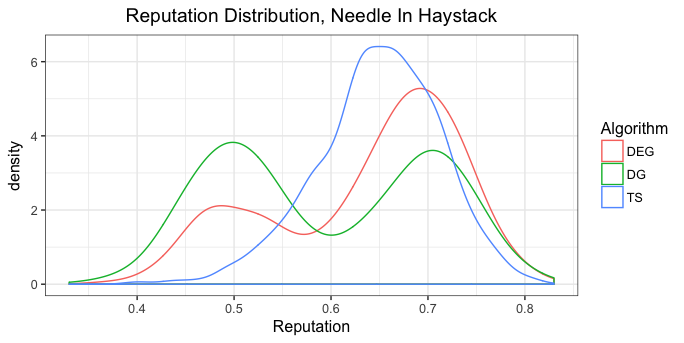
\includegraphics[scale=0.35]{figures/rep_distribution_nih}
\label{rep_dist_nih}
\caption*{\tiny{The plots contain a kernel density estimate of the reputation distribution at $t = 200$}}
\end{figure}

This motivates looking at the entire distribution of reputation difference between two algorithms. Figure \ref{ts_dg_rep_diff_nih} shows the distribution of reputation difference between $TS$ and $DG$ across $t$. This figure seems to confirm the intuition noted previously since the reputation distribution has its largest mass around the point just below 0 but it is skewed to the right even as $t$ gets large. Thus, the mean is not a representative statistic of the entire reputation difference distribution. As an alternative statistic for understanding the results of the competition game we introduce the \textit{relative reputation proportion} which looks at the proportion of simulations in which algorithm $A$ had at least as high of a reputation as algorithm $B$ for a fixed time $t$. This corresponds to running the bandit algorithms in isolation on the same instance and with the same realizations for $t$ rounds and then calculating the fraction of simulations at which an agent would select a firm playing $A$ over a firm playing $B$ at time $t$ \footnote{Though we do not discuss it here, one may be interested in if there is ever a case where, for sufficiently large $t$, we observe that $DEG >DG$ or $TS > DG$ according to the mean reputation but $DG > DEG$ or $DG > TS$ according to the relative reputation proportion. In the GitHub appendix we have results showing that, for Heavy Tail prior with $K=3$ we have that $DEG > DG$ according to the mean reputation but $DG > DEG$ according to the relative reputation proportion. Additionally, these results carry over to the competition game}.

\begin{figure}
\caption{Reputation Difference Distribution}
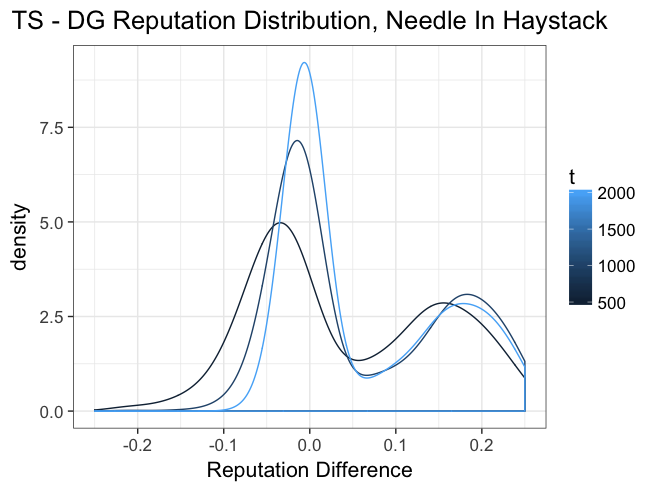
\includegraphics[scale=0.35]{figures/ts_dg_rep_diff_nih}
\label{ts_dg_rep_diff_nih}
\caption*{\tiny{The plots contain a kernel density estimate of the difference in reputation between $TS$ and $DG$ across $t$}}
\end{figure}

Figure \ref{relative_rep_plots} shows plots of the relative reputation proportion for $TS$ vs $DG$ on the Uniform and Needle In Haystack prior. For the Uniform prior we see that, in the early rounds, $DG > TS$ for the majority of the simulations but that, eventually, $TS > DG$. The intuition behind this is that, especially since the firms start with no substantive initial information, $TS$ does purposeful exploration in the early rounds in order to acquire information. However, this exploration leads to what we define as a \textit{relative reputation cost}. Namely, exploration leads to lower reputation relative to the myopic alternative. However, eventually the information acquired in the early rounds allows $TS$ to make better decisions and achieve a higher reputation, especially when the instance is ``hard enough" so that $DG$ cannot trivially find the best arm. We define this as the \textit{relative reputation benefit} \footnote{We see similar behavior for the Heavy Tail prior}.

\begin{figure}
\caption{Relative Reputation Plots}
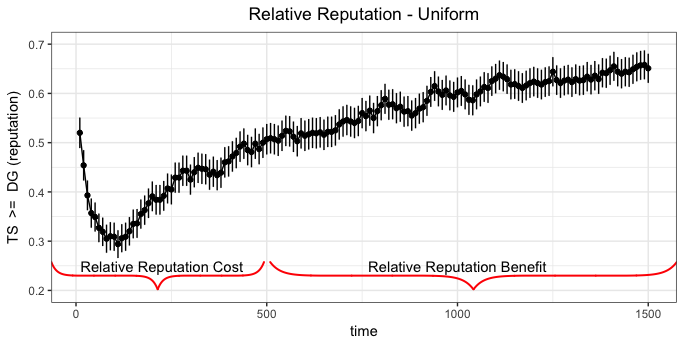
\includegraphics[scale=0.35]{figures/relative_uniform_annotated_plot}
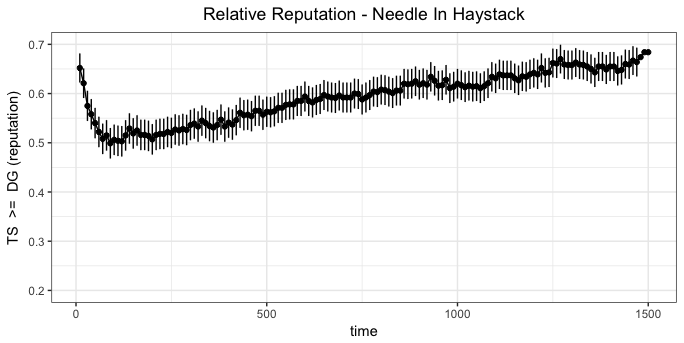
\includegraphics[scale=0.35]{figures/ts_dg_nih_10_prelim}
\caption*{\tiny{The plots contain the average reputation over $1000$ runs for a memory size of $100$ where, for a given $t$, we record the reputation of both of the algorithms on a given instance and then calculate the proportion of runs where $TS \geq DG$. The shaded area display 95\% confidence intervals.}}
\label{relative_rep_plots}

\end{figure}

Is exploration always costly? Figure \ref{relative_rep_plots} also shows that for the Needle In Haystack prior, $TS$ always does relatively better than $DG$. There are two contributing factors to this. First, $TS$ identifies the best arm faster in the Needle In Haystack prior than the Uniform prior so that there is a shorter time horizon where $TS$ needs to engage in purposeful exploration. Second, in the Needle In Haystack prior there are no ``bad" arms as there may be in the Uniform prior since by construction all the arms except one in Needle In Haystack are the same. Thus, when $TS$ pulls a sub-optimal arm relative to its current information, the expected reward is the same as the greedy option that has not identified the best arm. However, with the Uniform prior, it is possible that the sub-optimal arm that is pulled has substantially lower expected reward relative to the greedy option.

\section{Competition vs Better Algorithms: Inverted-U}
\label{S:5}

In this section we document our main results that can be summarized via the empirically documented inverted-U relationship between competition and innovation described in \citet{aghion2005competition}. We consider three separate settings for our model: permanent monopoly, temporary monopoly (incumbent vs entrant), and permanent duopoly. In the permanent monopoly and permanent duopoly cases we show that, under certain conditions, firms are incentivized to commit to $DG$ whereas in the temporary monopoly case firms are incentivized to commit to $TS$. We interpret the move from permanent monopoly to temporary monopoly and temporary monopoly to permanent duopoly as increases in competition. We believe this is reasonable and consistent with the empirical results which define increases in competition as increases in a measure of market power (1 - the Lerner Index). In our model we have no prices and no costs and so we interpret increases in ``market power" as decreases in the number of rounds where a firm has to compete for agents.

We utilize the same instances and realizations as in the section~\ref{S:3} and simulate the model described in section~\ref{S:2}. We initially take the strategies of the firms as exogenous (chosen from $\mathcal{A}$) and simulate the model given these strategies in order to determine the expected payoffs associated with each pair of algorithms. Unless otherwise noted, all the results are reported at $t = 2000$.

\textbf{Permanent Monopoly} Under permanent monopoly only a single firm exists in the market for every period. Since, in our formulation, the firm only gets utility from a larger market share it is indifferent between each algorithm in $\mathcal{A}$ since, regardless of the algorithm it deploys, it will get the entire market. If we suppose that deploying the ``better" algorithms has even an $\epsilon > 0$ cost, then the firm would choose to deploy $DG$.

\textbf{Permanent Duopoly} Permanent duopoly corresponds to the model described in section~\ref{S:2} where $X = 0$ so that both firms enter the market simultaneously. What algorithms are firms incentivized to deploy? We report the average market share taken over the $N$ simulations for a set of exogenous values of $k$. Additionally, we report the mean and median of an additional quantity which we define as the effective end of game.

\begin{definition}
\textit{Effective End of Game (EEOG)} - the last round, $t$, in a simulation where the agent alive at $t-1$ and the agent alive at $t$ choose different firms.
\end{definition}

Since both firms enter at the same time the game is symmetric and we only need to compute the payoffs of three pairs of strategies. We do not report them in the figures, but when both firms play the same algorithm the expected market share is 50/50. Tables \ref{sim_nih}, \ref{sim_ht}, and \ref{sim_unif} report the results.
\begin{enumerate}
\item Under Needle In Haystack we have that $TS$ always does weakly better than $DEG$ and $DG$, regardless of the warm start
\item Under Heavy Tail we have that, for low warm start, $DEG, DG > TS$ but that for the higher warm start values we consider $TS > DEG, DG$. Interestingly, even under the relatively high warm start we see $DG > DEG$.
\item Under Uniform we have that $DEG, DG > TS$ for low warm start and $TS > DEG, DG$ for sufficiently high warm start.
\end{enumerate}

Looking at the relative reputation plots in Figure \ref{relative_rep_plots}, we can interpret fixing a warm start value as fixing the starting point on the relative reputation plots. The proportion of first rounds in the competition game that will go to a firm playing alg $A$ over a firm playing alg $B$ will correspond to the relative reputation proportion at time $k$. Combined with the fact that the EEOG values being relatively low across all warm starts \footnote{Interestingly, the EEOG also appears to be skewed to the right, similar to the distribution of reputation differences}, these observations seem to imply that understanding the performance of different algorithms in competition it is important to look at their performance for relatively small samples instead of asymptotically.

For the low values of the warm start we can see that $DG > TS$ for the Uniform prior but $TS > DG$ for the Needle In Haystack prior and this corresponds to what we see in the relative reputation proportion plots. The intuition for this result aligns with the intuition given in the discussion of the relative reputation plots. Namely, for low warm start values $TS$ incurs a relative reputation cost compared to $DG$ since it engages in purposeful exploration. Moving to a sufficiently large warm start so that the better algorithm has recovered from the relative reputation cost incurred via exploration leads to better algorithms winning. However, it appears that the warm starts required for this are unreasonably high, especially for the Uniform prior.

Focusing on reasonable warm starts, $DG > TS$ when it appears that better algorithms suffer an early relative reputational cost due to exploration and that both firms enter at the same time so that there is a ``permanent duopoly."

\begin{table}[ht]
\centering
\caption{Duopoly Experiment Needle In Haystack} 
\begin{tabular}{rlll}
  \hline
 & k = 20 & k = 250 & k = 500 \\ 
  \hline
TS vs DG & \makecell{\textbf{0.64} $\pm$0.03\\ eeog \\ avg: 200\\ med: 27} & \makecell{\textbf{0.6} $\pm$0.03\\ eeog \\ avg: 370\\ med: 0} & \makecell{\textbf{0.64} $\pm$0.03\\ eeog \\ avg: 580\\ med: 121.5} \\ 
  TS vs DEG & \makecell{\textbf{0.57} $\pm$0.03\\ eeog \\ avg: 150\\ med: 14} & \makecell{\textbf{0.52} $\pm$0.03\\ eeog \\ avg: 460\\ med: 78.5} & \makecell{\textbf{0.56} $\pm$0.02\\ eeog \\ avg: 740\\ med: 627.5} \\ 
  DG vs DEG & \makecell{\textbf{0.46} $\pm$0.03\\ eeog \\ avg: 340\\ med: 128.5} & \makecell{\textbf{0.42} $\pm$0.02\\ eeog \\ avg: 650\\ med: 408} & \makecell{\textbf{0.42} $\pm$0.02\\ eeog \\ avg: 690\\ med: 466.5} \\ 
   \hline
\end{tabular}
\label{sim_nih}
\caption*{\tiny{The first line in each cell contains the average market share received by the firm playing Alg 1 (and the market share of Alg 2 is 1 - Alg 1 Market Share) as well as a 95 \% confidence band. For example, the cell in the top left indicates that TS gets on average 64\% of the market when played against DG. The next line contain the average and median effective end of game for this set of simulations.}}
\end{table}
% latex table generated in R 3.4.0 by xtable 1.8-2 package
% Thu Aug 16 13:13:00 2018
\begin{table}[ht]
\centering
\caption{Duopoly Experiment Heavy Tail} 
\begin{tabular}{rlll}
  \hline
 & k = 20 & k = 250 & k = 500 \\ 
  \hline
TS vs DG & \makecell{\textbf{0.29} $\pm$0.03\\ eeog \\ avg: 55\\ med: 0} & \makecell{\textbf{0.72} $\pm$0.02\\ eeog \\ avg: 570\\ med: 0} & \makecell{\textbf{0.76} $\pm$0.02\\ eeog \\ avg: 620\\ med: 98.5} \\ 
  TS vs DEG & \makecell{\textbf{0.3} $\pm$0.03\\ eeog \\ avg: 37\\ med: 0} & \makecell{\textbf{0.88} $\pm$0.01\\ eeog \\ avg: 480\\ med: 0} & \makecell{\textbf{0.9} $\pm$0.01\\ eeog \\ avg: 570\\ med: 113.5} \\ 
  DG vs DEG & \makecell{\textbf{0.62} $\pm$0.03\\ eeog \\ avg: 410\\ med: 7} & \makecell{\textbf{0.6} $\pm$0.02\\ eeog \\ avg: 790\\ med: 762} & \makecell{\textbf{0.57} $\pm$0.03\\ eeog \\ avg: 730\\ med: 608} \\ 
   \hline
\end{tabular}
\label{sim_ht}
\end{table}
% latex table generated in R 3.4.0 by xtable 1.8-2 package
% Thu Aug 16 13:13:01 2018
\begin{table}[ht]
\centering
\caption{Duopoly Experiment Uniform} 
\begin{tabular}{rlll}
  \hline
 & k = 20 & k = 250 & k = 500 \\ 
  \hline
TS vs DG & \makecell{\textbf{0.46} $\pm$0.03\\ eeog \\ avg: 230\\ med: 0} & \makecell{\textbf{0.52} $\pm$0.02\\ eeog \\ avg: 800\\ med: 754} & \makecell{\textbf{0.6} $\pm$0.02\\ eeog \\ avg: 910\\ med: 906.5} \\ 
  TS vs DEG & \makecell{\textbf{0.41} $\pm$0.03\\ eeog \\ avg: 180\\ med: 0} & \makecell{\textbf{0.51} $\pm$0.02\\ eeog \\ avg: 810\\ med: 734} & \makecell{\textbf{0.55} $\pm$0.02\\ eeog \\ avg: 970\\ med: 987} \\ 
  DG vs DEG & \makecell{\textbf{0.51} $\pm$0.03\\ eeog \\ avg: 470\\ med: 57.5} & \makecell{\textbf{0.48} $\pm$0.02\\ eeog \\ avg: 1000\\ med: 1088} & \makecell{\textbf{0.45} $\pm$0.02\\ eeog \\ avg: 1000\\ med: 1142} \\ 
   \hline
\end{tabular}
\label{sim_unif}
\end{table}

\textbf{Temporary Monopoly} We now consider asymmetries in the timing of entry so that one firm enters the market before the other and serves as a monopolist in the periods until the other firm enters. In terms of our model, this corresponds to setting $X = 200$. For this section we report results fixing $k = 20$. Does this lead the incumbent to commit to $TS$? How about the entrant? 

Table \ref{ht_incum} shows the results of the simulations for this parameterization. We observe that, for the incumbent, $TS$ is the dominant strategy across all priors. In the appendix we include additional simulations where $X = 50$ and observe that $TS$ is not always a dominant strategy in this case. This result is robust across all of the priors that we considered so that for sufficiently large $X$, $TS$ is a dominant strategy for the incumbent where $X$ depends on the set of instances that we are considering.

% latex table generated in R 3.4.0 by xtable 1.8-2 package
% Wed Aug 15 19:03:20 2018
\begin{table}[ht]
\centering
\caption{Temporary Monopoly Experiment Heavy Tail} 
\begin{tabular}{c@{\hspace{1.0\tabcolsep}}ccc}
  \hline
 & TS & DEG &  DG \\ 
  \hline
TS & \makecell{\textbf{ 0.0029 } $\pm$ 0.003 \\Var: 0.002 \\ ES: 100 \%} & \makecell{\textbf{ 0.11 } $\pm$ 0.02 \\Var: 0.09 \\ ES: 96 \%} & \makecell{\textbf{ 0.17 } $\pm$ 0.02 \\Var: 0.1 \\ ES: 95 \%} \\ 
  DEG & \makecell{\textbf{ 0.049 } $\pm$ 0.01 \\Var: 0.03 \\ ES: 94 \%} & \makecell{\textbf{ 0.24 } $\pm$ 0.02 \\Var: 0.1 \\ ES: 74 \%} & \makecell{\textbf{ 0.24 } $\pm$ 0.02 \\Var: 0.1 \\ ES: 79 \%} \\ 
   DG & \makecell{\textbf{ 0.12 } $\pm$ 0.02 \\Var: 0.08 \\ ES: 87 \%} & \makecell{\textbf{ 0.35 } $\pm$ 0.03 \\Var: 0.2 \\ ES: 77 \%} & \makecell{\textbf{ 0.29 } $\pm$ 0.02 \\Var: 0.1 \\ ES: 65 \%} \\ 
   \hline
\end{tabular}
\caption*{\tiny{The columns represent the strategy of the incumbent and the rows represent the strategy of the entrant. The first line in each cell contains the average market share for the entrant over $N=1000$ simulations as well as a 95\% confidence interval. The second line contains the sample variance of the observed market shares and the third line contains the fraction of simulations that ended up with one firm getting $> 90\%$ of the market. Note that smaller values in the table are better for the incumbent. Market shares are calculated as the fraction of users selecting a particular firm \textit{after} the entrant has already entered (i.e. the free rounds to firm 2 do not count towards the share)}}
\label{ht_incum}
\end{table}
Why do we observe that $TS$ is the dominant strategy for the incumbent whereas in the permanent duopoly experiment we saw that, for this warm start, $DG$ was preferred to $TS$? The intuition for this is that competition in the duopoly forces the firms to worry about their reputation which dissuades them from committing to algorithms that involve pure exploration in the early rounds. This intuition is very similar to that observed in the previous section by increasing warm start. In some sense one can view allowing one firm to temporarily be a monopolist as temporarily relaxing the ``incentive" component of exploration, exploitation, and incentives so that the incumbent firm only faces the classic tradeoff between exploration and exploitation. The incumbent only needs to worry about her reputation after $X$ periods when the entrant comes into the market and again needs to worry about incentivizing agents to select them over their competition. As a result, the incumbent is incentivized to commit to an algorithm that does exploration in the early rounds since she no longer suffers the same relative reputational cost that she would suffer under competition as long as the $X$ is sufficiently large that she can begin to recover the reputational costs of exploration. Thus, counterintuitively, by having one firm be a monopoly and dominate the market, we can incentivize them to play $TS$.

What about for the entrant? We do not find that $TS$ is a dominant strategy, though $TS$ is not dominated by $DG$. Since the game we consider is a zero-sum game, there exists equililibria where $TS$ is played with some positive probability in equilibrium.

\section{Data and Reputation as Barriers to Entry}
\label{S:6}

An alternative interpretation of the results in the previous section is that the ``temporary monopoly" provides a first mover advantage to the incumbent firm and that this first mover advantage allows the firm to both get a data advantage as well as a reputational advantage over the entrant. This provides an alternative interpretation of the classic ``first mover advantage" that has been well-studied in economics and marketing \citep*{kerin1992first} where, in our model, an incumbent can use data and reputation as a barrier to entry. Which plays a bigger role in preventing the entrant from being able to establish market share? We run two additional experiments, modifying the previous incumbent experiment so that in one set of simulations the reputation of the incumbent is artificially erased and another in which the information gained by the incumbent is artificially erased so that the posterior is reset to the prior.

\begin{table}[ht]
\centering
\caption{Reputation Erased Experiment, Heavy Tail} 
\begin{tabular}{c@{\hspace{1.0\tabcolsep}}ccc}
  \hline
 & TS & DEG &  DG \\ 
  \hline
TS & \makecell{\textbf{ 0.016 } $\pm$ 0.0075 \\Var: 0.01 \\ ES: 100 \%} & \makecell{\textbf{ 0.13 } $\pm$ 0.02 \\Var: 0.1 \\ ES: 97 \%} & \makecell{\textbf{ 0.2 } $\pm$ 0.024 \\Var: 0.1 \\ ES: 96 \%} \\ 
  DEG & \makecell{\textbf{ 0.068 } $\pm$ 0.013 \\Var: 0.05 \\ ES: 93 \%} & \makecell{\textbf{ 0.29 } $\pm$ 0.024 \\Var: 0.2 \\ ES: 75 \%} & \makecell{\textbf{ 0.26 } $\pm$ 0.024 \\Var: 0.2 \\ ES: 80 \%} \\ 
   DG & \makecell{\textbf{ 0.15 } $\pm$ 0.019 \\Var: 0.1 \\ ES: 87 \%} & \makecell{\textbf{ 0.38 } $\pm$ 0.028 \\Var: 0.2 \\ ES: 80 \%} & \makecell{\textbf{ 0.33 } $\pm$ 0.024 \\Var: 0.2 \\ ES: 67 \%} \\ 
   \hline
   \label{rep_erase}
\end{tabular}
\end{table}
% latex table generated in R 3.4.0 by xtable 1.8-2 package
% Sun Jul 22 14:23:06 2018
\begin{table}[ht]
\centering
\caption{Information Erased Experiment, Heavy Tail} 
\begin{tabular}{c@{\hspace{1.0\tabcolsep}}ccc}
  \hline
 & TS & DEG &  DG \\ 
  \hline
TS & \makecell{\textbf{ 0.024 } $\pm$ 0.0094 \\Var: 0.02 \\ ES: 100 \%} & \makecell{\textbf{ 0.16 } $\pm$ 0.022 \\Var: 0.1 \\ ES: 97 \%} & \makecell{\textbf{ 0.22 } $\pm$ 0.025 \\Var: 0.2 \\ ES: 95 \%} \\ 
  DEG & \makecell{\textbf{ 0.24 } $\pm$ 0.025 \\Var: 0.2 \\ ES: 94 \%} & \makecell{\textbf{ 0.29 } $\pm$ 0.024 \\Var: 0.1 \\ ES: 72 \%} & \makecell{\textbf{ 0.27 } $\pm$ 0.024 \\Var: 0.1 \\ ES: 76 \%} \\ 
   DG & \makecell{\textbf{ 0.33 } $\pm$ 0.028 \\Var: 0.2 \\ ES: 94 \%} & \makecell{\textbf{ 0.38 } $\pm$ 0.026 \\Var: 0.2 \\ ES: 74 \%} & \makecell{\textbf{ 0.33 } $\pm$ 0.023 \\Var: 0.1 \\ ES: 58 \%} \\ 
   \hline
   \label{info_erase}
\end{tabular}
\end{table}

Tables \ref{rep_erase} and \ref{info_erase} display the results of these experiments. Maintaining the data or reputation advantage alone still allows the incumbent to retain a significant portion of the market. Interestingly, when the incumbent plays $DEG$ or $DG$ reputation and information serve as substitutes (the market shares are almost identical), but when the incumbent plays $TS$ information serves as a larger barrier to entry than reputation. This is robust across the priors that we consider for this parametrization. One possible intuition for this is that, for Heavy Tail, the information acquired after the $X$ rounds under $TS$ is sufficient so that it becomes relatively easier for $TS$ to recover the reputation loss compared to the information loss, but since $DEG$ and $DG$ learn slower and they've acquired less information over the $X$ rounds relative to $TS$ there is less of an informational advantage.

Though the setup is purely experimental, it is nonetheless interesting to look at if $TS$ still remains a dominant strategy for the incumbent. In the reputation erased experiment, $TS$ is still a dominant strategy while in the information erased experiment it is not a dominant strategy.

\bibliography{refs}

\end{document}
